\chapter{Implementación}\label{chap:implementación}
Para la implementación de la solución utilizaremos una arquitectura cliente-servidor\cite{client-server}, la cual nos
permite tener los datos centralizados en una aplicación servidor. La aplicación cliente realizará peticiones al
servidor, para que este le provea de los datos que necesite en cada momento.

\section{Servidor}
En el lado del servidor o \textit{back-end} se encuentra la mayor parte de la lógica de la aplicación, dedicándose el
lado del cliente a simplemente mostrarla en una interfaz cómoda para el usuario.\\

Se ha implementado un servidor que provee a los clientes de un listado de series y sus temporadas, así como de la
posibilidad de crear reseñas de las mismas o obtener las reseñas de otros usuarios.

\subsection{Lenguaje de programación}
El lenguaje de programación seleccionado para el servidor es \textit{Python}\cite{python}, ya que es un lenguaje de
programación que nos provee de una buena experiencia de desarrollo al ser un lenguaje menos estricto y cuenta con muchas
librerías útiles y una enorme comunidad a sus espaldas.\\

Uno de sus puntos débiles, es que al ser un lenguaje no tipado, es más propenso a errores de sintaxis, pero desde la
versión 3.5, cuenta con una forma de tipar el código, de forma que, aunque el intérprete de \textit{Python} no detecte
este tipado, puede ser utilizado por herramientas de los \textit{IDEs} y \textit{linters} para la detección precoz
errores.\\

Otro de los motivos que me han llevado a decantarme por este lenguaje son sus librerías científicas y de procesamiento
de datos. Con ellas, en un futuro podríamos incluir en la aplicación alguna herramienta para obtener estadísticas y
realizar predicciones sobre nuestros datos. Algo muy útil para un cliente que quiera usar los datos de la aplicación
para saber qué tipo de series interesan a cierto tipo de público, por ejemplo.\\

Como gestor de paquetes y dependencias, utilizo \textit{poetry}\cite{poetry}, que nos permite gestionar las dependencias
del proyecto de forma muy sencilla y similar a \textit{NPM}\cite{npm}.

\subsection{Framework}
El framework utilizado para el servidor es \textit{Flask}\cite{flask}, un framework de Python que nos permite una 
\textit{REST API}\cite{rest} minimalista, flexible y fácil de usar.

\subsection{Operaciones}
Recopilación y breve descripción de las peticiones que atiende el servidor.

\subsubsection{Autenticación}
Los usuarios podrán loguearse con su cuenta, lo que generará un token de acceso que deberá ser enviado en las cabeceras
del resto de peticiones, para identificar qué usuario está realizando la petición, lo que en algunas de las operaciones
será obligatorio.\\

Para asegurarnos que el usuario está logueado, utilizamos un \textit{decorador} de la librería
\textit{Flask-JWT-Extended}\cite{jwt} que comprueba que el token enviado en las cabeceras de la petición es válido. Si
no lo es, se devuelve un error 401, o de desautorización.

\subsubsection{Series}
El servidor provee de una lista de series o de los detalles de una serie en particular o alguna de sus temporadas a
través de su identificador. Sin embargo, la base de datos no incluye la información de estas series, si no que se
obtienen a través de una API externa.\\

La API utilizada es \href{https://www.themoviedb.org}{\textit{TheMovieDB}}, una API abierta que provee de datos sobre
series y películas. En este caso, haremos uso de las series. Gracias al diseño de nuestra aplicación, podríamos cambiar
de API en cualquier momento, sin que suponga mucho tiempo de desarrollo.\\

Además, también provee de una lista de series ordenadas por popularidad, según los rankings de \textit{TheMovieDB}.

\subsubsection{Usuarios}
Cualquiera podrá listar o crear un usuario, siempre y cuando el email introducido no esté en uso.\\

A través de su ID, se podrán acceder a los datos de dicho usuario u obtener las reseñas que ha realizado.\\

Además, los usuarios identificados podrán seguir o dejar de seguir a otros usuarios y obtener la lista de reseñas hechas
por cualquier de los usuarios que están siguiendo.

\subsubsection{Reseñas}
Los usuarios identificados podrán crear reseñas de las series. Usando el token \textit{JWT} del que hablamos en la
sección anterior, podemos obtener el identificador del usuario que está realizando la petición y añadirlo a los datos de
la reseña.\\ 

Además, cualquier usuario - identificado o no - podrá obtener la lista de reseñas hechas en la aplicación, ordenadas de
más a menos recientes.

\subsection{Test}
Como ya hablamos en la \hyperref[chap:metodología]{metodología}, necesitamos que el código cumpla con unos requisitos
mínimos de calidad a través de \textit{tests}.\\

Para el servidor, se han implementado tests unitarios con la librería \textit{pytest}\cite{pytest}, que comprueban que
los métodos de los modelos de la aplicación funcionan correctamente.

\begin{figure}[H]
\centering	
    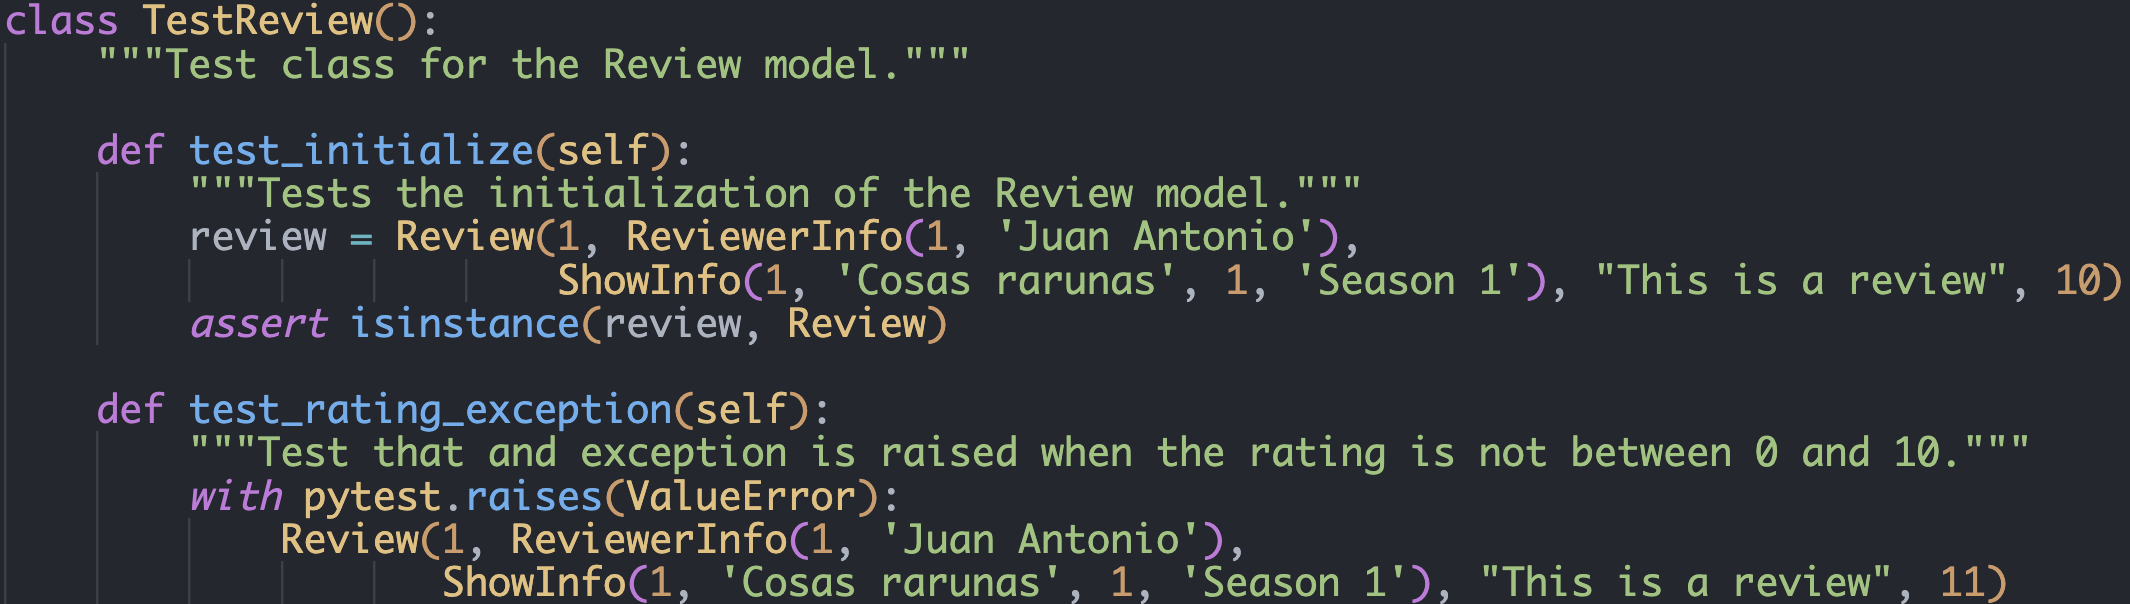
\includegraphics[scale=0.25]{img/pytest.png}
\caption{ Test unitario de la clase Show en Python }\label{fig:pytest}
\end{figure}

\subsection{Base de datos}
El número de reseñas irá en aumento con el tiempo y con el número de usuarios de la aplicación, por lo que necesito una
base de datos que sea fácilmente escalable. Por ello, \textit{MongoDB}\cite{mongodb} es una muy buena opción, gracias a
\textit{MongoAtlas}\cite{mongoatlas}, una herramienta \textit{DataBase as a Service}\cite{dbaas} que nos permite escalar
la base de datos verticalmente, aumentando el poder de procesamiento de nuestro cluster, u horizontalmente, añadiendo
más nodos para compartir la carga.\\

Además, guarda los datos en formato \textit{JSON}\cite{json}, lo que nos permite acceder a ellos de forma muy sencilla y
fácilmente interpretable por cualquier lenguaje de programación moderno.

\subsection{Configuración}
Las variables de configuración se encuentran en los ficheros del directorio \textit{config} y se definen mediante las
variables de entorno, incluyendo opciones por defecto en la mayoría. En el entorno de desarrollo, uso \textit{dotenv}
para cargar las variables de entorno desde un fichero de configuración \textit{.env}.

\begin{figure}[H]
\centering	
    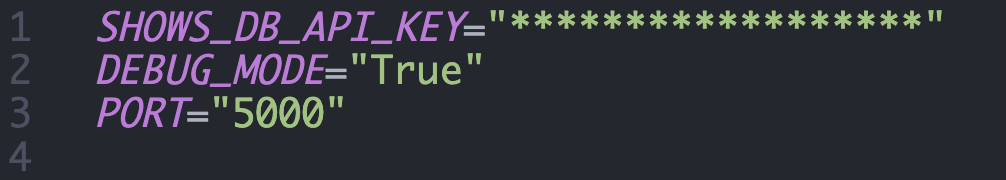
\includegraphics[scale=0.525]{img/dotenv.png}
\caption{ Fichero de configuración con las variables de entorno del servidor }\label{fig:dotenv}
\end{figure}

Para el entorno de producción, las variables se cargan en \textit{Heroku}\cite{heroku} de forma sencilla, como veremos
en el \hyperref[sec:despliegue]{despliegue}.

\section{Cliente}
El cliente o \textit{back-end} es la parte de la aplicación que se ejecuta en el dispositivo del usuario. En nuestro
caso, la mayor parte de la lógica se encuentra en el lado del servidor y el cliente se encarga de mostrar la información
y dar acceso a las peticiones del servidor de una forma amigable para el usuario.

\subsection{Elección de la tecnología}
Con el paso del tiempo, cada vez más frameworks y librerías se han ido desarrollando para la creación de aplicaciones
cliente, por lo que hay una gran variedad de tecnologías a nuestra disposición.

\subsubsection{Aplicación web vs aplicación móvil}
Es cierto que las aplicaciones móviles están ganando cada vez más popularidad, ya que con la afluencia de dispositivos
inteligentes como teléfonos, tablets, televisores e incluso frigoríficos, es más fácil acceder a la información desde
cualquier parte.\\

No por ello, debemos descartar las aplicaciones web. En este caso, una aplicación web es una solución sólida al
problema, al ser más cómodo para los usuarios escribir sus reseñas con su teclado y ratón, y no con su pantalla
táctil.

\subsubsection{Frameworks}
Los tres grandes framework para aplicaciones web son: \textit{Angular}\cite{angular}, \textit{React}\cite{react} y
\textit{Vue}\cite{vue}.\\

\noindent \textbf{Vue}\\ \\
\indent \textit{Vue} es un framework muy ligero, que se basa en componentes, lo que lo hace muy fácil de aprender y de usar.
Además, permite usar expansiones de terceros para añadir componentes o funcionalidades hechas por la comunidad. Sin
embargo, utiliza \textit{JavaScript}\cite{javascript} como lenguaje de programación, por lo que no es la opción más
deseable frente a los otros dos.\\

\noindent \textbf{React}\\ \\
\indent \textit{React} está basado en \textit{JavaScript} y utiliza \textit{JSX}\cite{jsx} para definir los componentes, aunque
también se puede usar \textit{TypeScript}\cite{typescript}, un lenguaje tipado que se transpila a \textit{JavaScript},
lo que nos permite la detección rápida de errores. Es un framework muy popular y con una gran comunidad detrás, lo que
lo convierte en una buena opción.\\

\noindent \textbf{Angular}\\ \\
\indent Finalmente, el framework que he elegido es \textit{Angular}. Aunque esté perdiendo popularidad, sigue
siendo una gran opción para el desarrollo de aplicaciones web. Trabaja nativamente con \textit{TypeScript}, por lo que
fácilmente podremos disfrutar de las ventajas de un lenguaje tipado.\\

\textit{Angular} es un framework diseñado y mantenido por \textit{Google} que nos ofrece un código bien estructurado
basado en componentes y servicios, que nos permite desarrollar con una arquitectura limpia y mantenible. Además, nos
permite usar \textit{Angular Material}\cite{angularmaterial}, un conjunto de componentes de \textit{Angular} que nos
permite crear interfaces de usuario modernas de forma rápida y sencilla y también cuenta con \textit{Ionic}\cite{ionic},
un framework para crear aplicaciones híbridas para móviles y web si en algún momento decidiésemos dar el salto a las
aplicaciones móviles.

\subsection{Diseño}
En esta sección se detallarán los aspectos de las diferentes vistas de la aplicación. Se ha apostado por un diseño
elegante y minimalista, usando los componentes del ya mencionado \textit{Angular Material}.

\subsubsection{Barra de navegación}
En la parte de arriba de cualquiera de las vistas de la aplicación, se encuentra la barra de navegación.\\

La barra de navegación muestra el título de la aplicación y otras dos pestañas: \textit{Shows} y \textit{Users}.\\

Hacer click en el título redirigirá al usuario a la feed principal de la aplicación, mientras que hacer click en
alguna de las otras dos vistas, le transportará a la lista de series y de usuarios, respectivamente.\\

En la parte derecha de la barra de navegación, nos encontraremos la pestaña de \textit{Log In}, que desplegará la
\hyperref[sec:login-signin]{ventana de registro y logueo}. En caso de ya estar logueado, la pestaña mostrará tu nombre de
usuario y haciendo click, desplegará un menú cuya única opción es el deslogueo.

\begin{figure}[H]
    \centering	
        
\includegraphics[scale=0.25]{img/navbar.png}
    \caption{ Barra de navegación previa al login }\label{fig:navbar}
\end{figure}

\begin{figure}[H]
    \centering	
        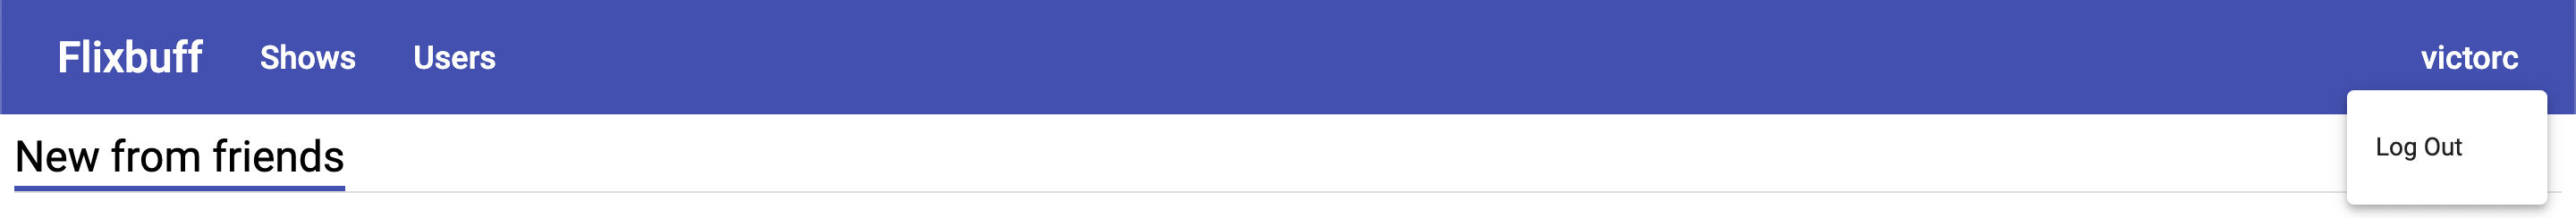
\includegraphics[scale=0.25]{img/logged-navbar.png}
    \caption{ Barra de navegación posterior al login }\label{fig:logged-navbar}
\end{figure}

\subsubsection{Ventana de login/registro}\label{sec:login-signin}
Tras el click en la pestaña de \textit{log in} se despliega esta ventana que se superpone al resto de la aplicación.\\

La ventana está dividida en tres secciones: las pestañas, el formulario y los botones. \\

Las dos pestañas son \textit{Log In} y \textit{Create Account} y modifican el resto de la ventana acorde a la operación
que quieras llevar a cabo, acceso o registro, respectivamente.\\

En la parte baja de la ventana encontramos dos botones, el primero refleja la acción que se intenta llevar a cabo - 
acceso o registro - y no funcionará hasta que los datos del formulario correspondiente sean correctos. El segundo botón
sirve para cancelar la operación y cerrar la ventana.

\begin{figure}[H]
    \centering	
        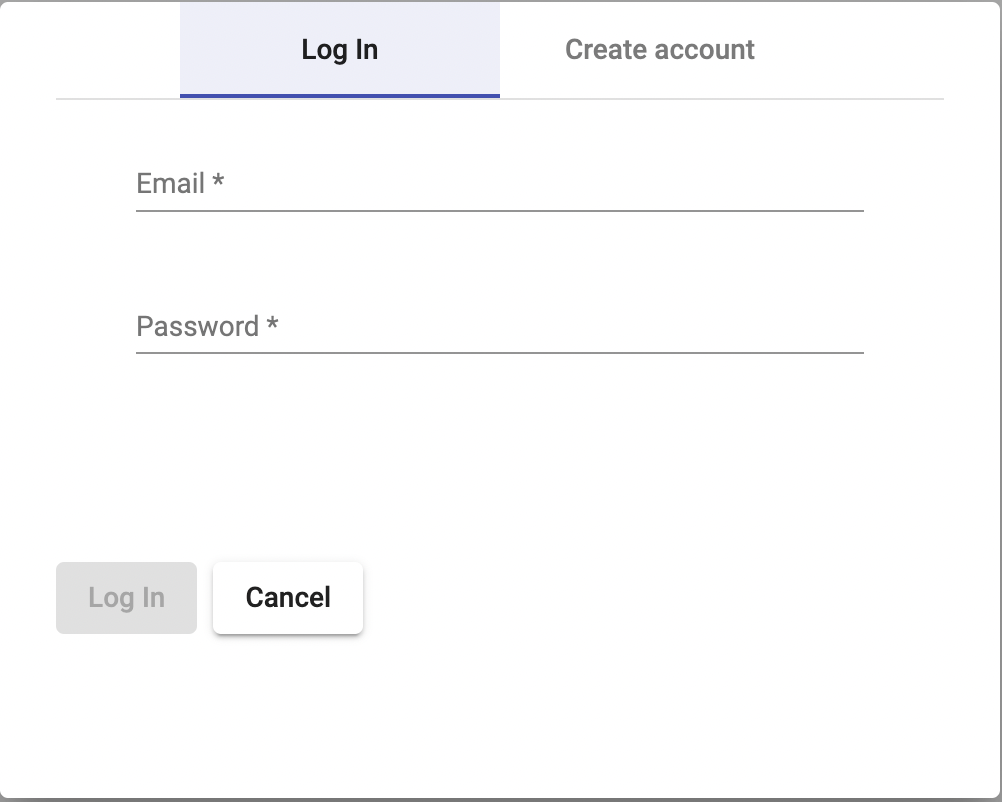
\includegraphics[scale=0.25]{img/login.png}
        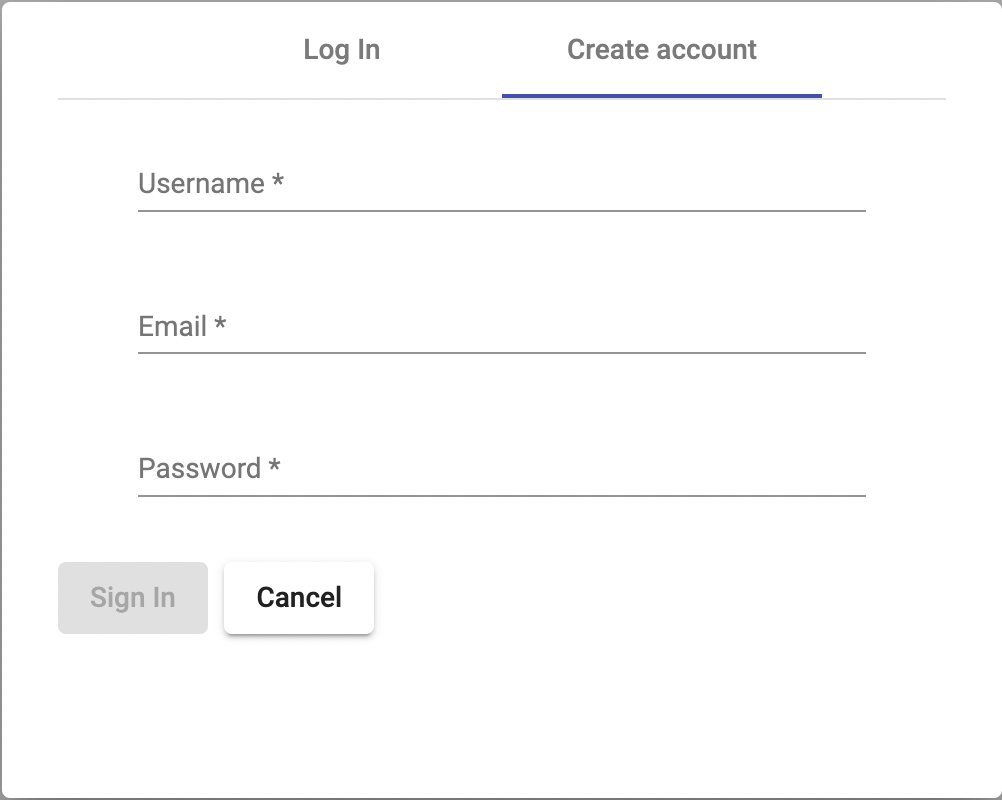
\includegraphics[scale=0.25]{img/signin.png}
    \caption{ Ventana de acceso y registro }\label{fig:login}
\end{figure}

\subsubsection{Feed principal}
El feed principal de la aplicación está compuesto por tres secciones.\\

La primera sección, solo visible a usuarios logueados, muestra las reseñas más recientes de los usuarios a los que
siguen. Las reseñas se muestran en un carrusel de tarjetas y unos botones a los lados que permiten cambiar de página.\\

Estas tarjetas tienen por título el título de la serie y el nombre de la temporada y el nombre del revisor como
subtítulo, acompañados por el texto de la reseña y su puntuación representada por estrellas. Además de el poster de la
temporada en la parte izquierda.

\begin{figure}[H]
    \centering	
        
\includegraphics[scale=0.5]{img/review-card.png}
    \caption{ Tarjeta de reseña }\label{fig:review-card}
\end{figure}

La segunda sección muestra las series más populares del momento, en forma de carrusel de tarjetas, al igual que con las
reseñas. En este caso, las tarjetas incluyen el título de la serie y su fecha, el póster de la obra y un pequeño resumen
de la misma. Hacer click en una serie te llevará a la vista de detalles de la misma.

\begin{figure}[H]
    \centering	
        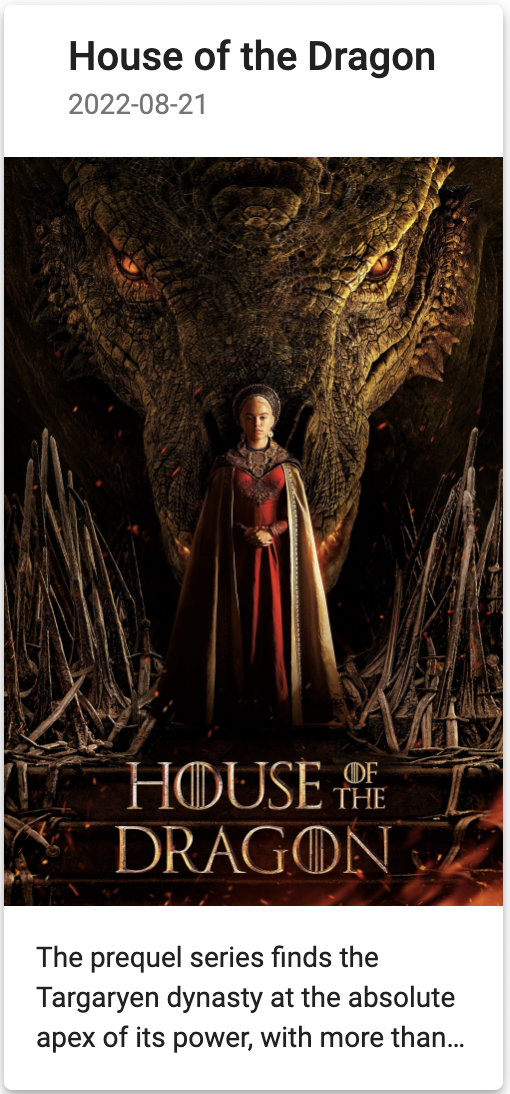
\includegraphics[scale=0.5]{img/show-card.png}
    \caption{ Tarjeta de serie }\label{fig:show-card}
\end{figure}

La tercera sección muestra lo mismo que la primera, pero en este caso muestra la reseñas más recientes de todos los
usuarios de la aplicación. Al hacer click en alguna de ellas, te llevará al perfil del usuario que la escribió, para que
puedas seguirle y ver sus otras reseñas.

\subsubsection{Lista de series}
En la lista de series podemos encontrar una barra de búsqueda en la parte superior de la vista. Al escribir algo en la
barra, automáticamente se buscarán las series que contengan esa cadena en el nombre y se mostrarán en una rejilla de
tarjetas de series como las de la sección anterior.\\

\begin{figure}[H]
    \centering	
        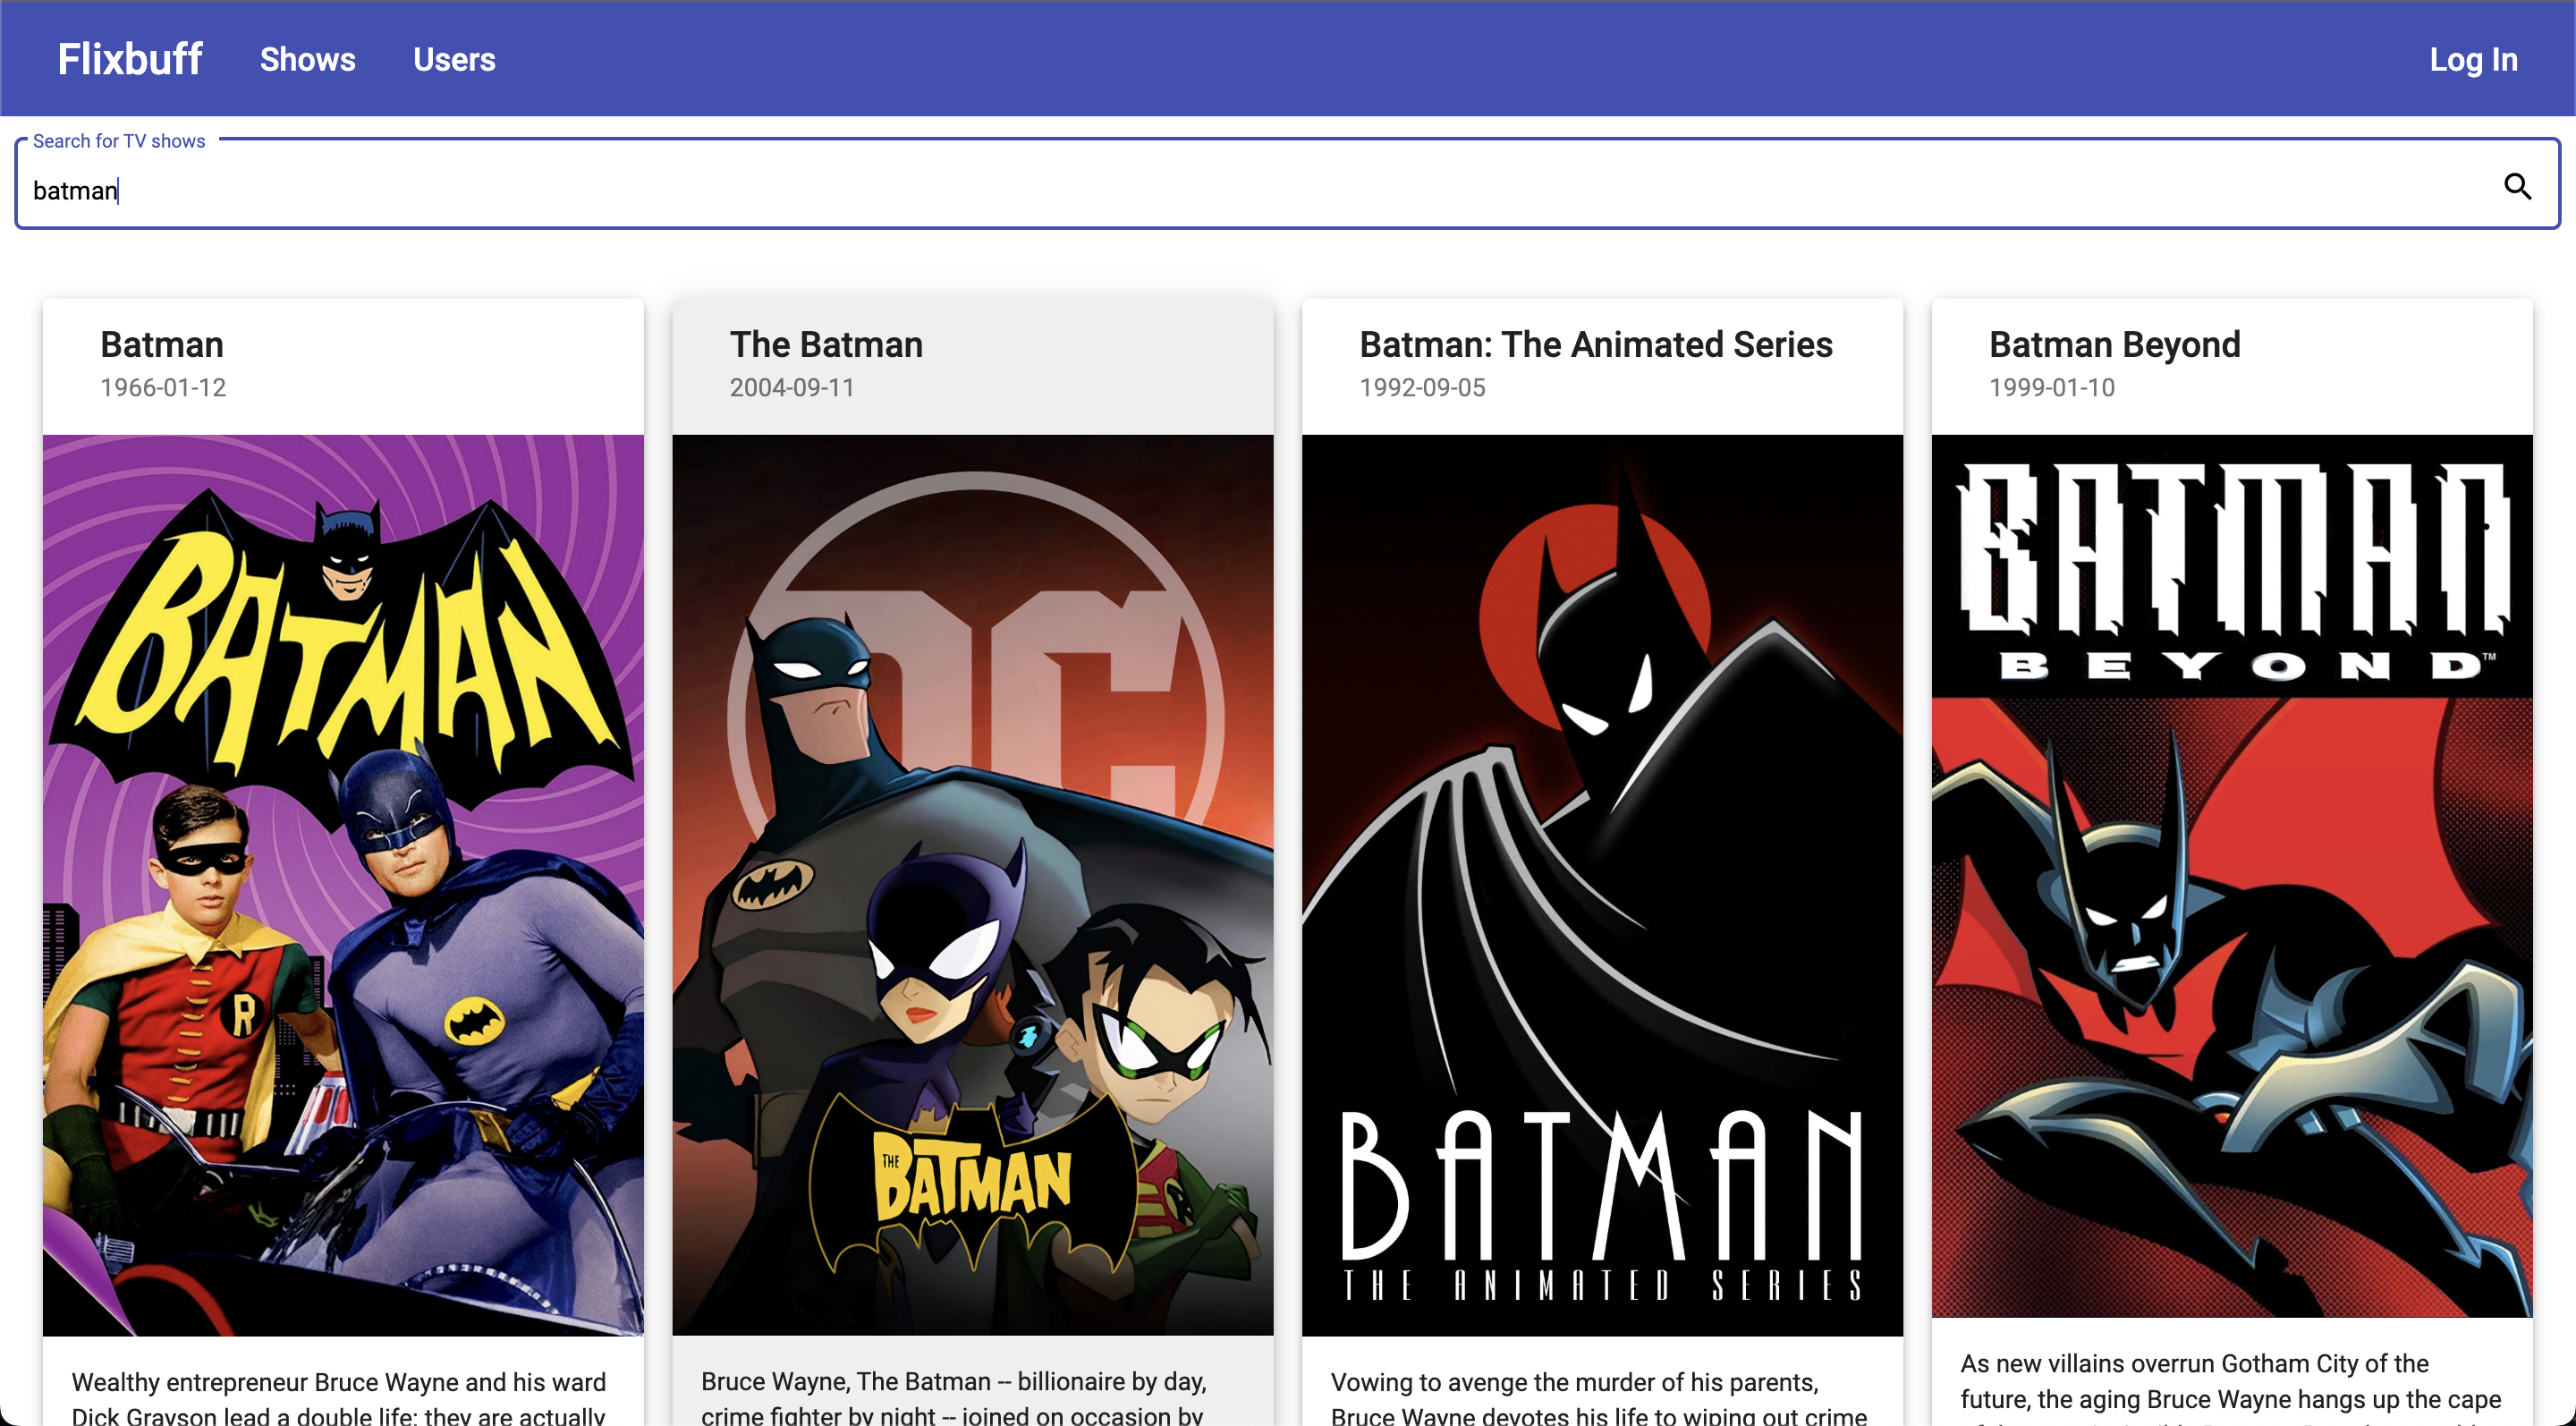
\includegraphics[scale=0.25]{img/show-list.png}
    \caption{ Lista de series con el nombre \textit{Batman} }\label{fig:show-list}
\end{figure}

Al igual que en la sección anterior, hacer click en una de las tarjetas te llevará a la vista de detalles de la serie.

\subsubsection{Detalles de una serie}
La vista de detalles de la serie nos muestra dos partes. \\

La primera parte es una cabecera con información de la serie, en la que, al igual que en la tarjeta, se podrán ver su
título, fecha de estreno, un pequeño resumen y una imagen de la misma.\\

La segunda parte está formada por la lista de sus temporadas, representadas en unas tarjetas expansibles, que al hacer
click sobre ellas, revelan más información sobre la misma.

\begin{figure}[H]
    \centering	
        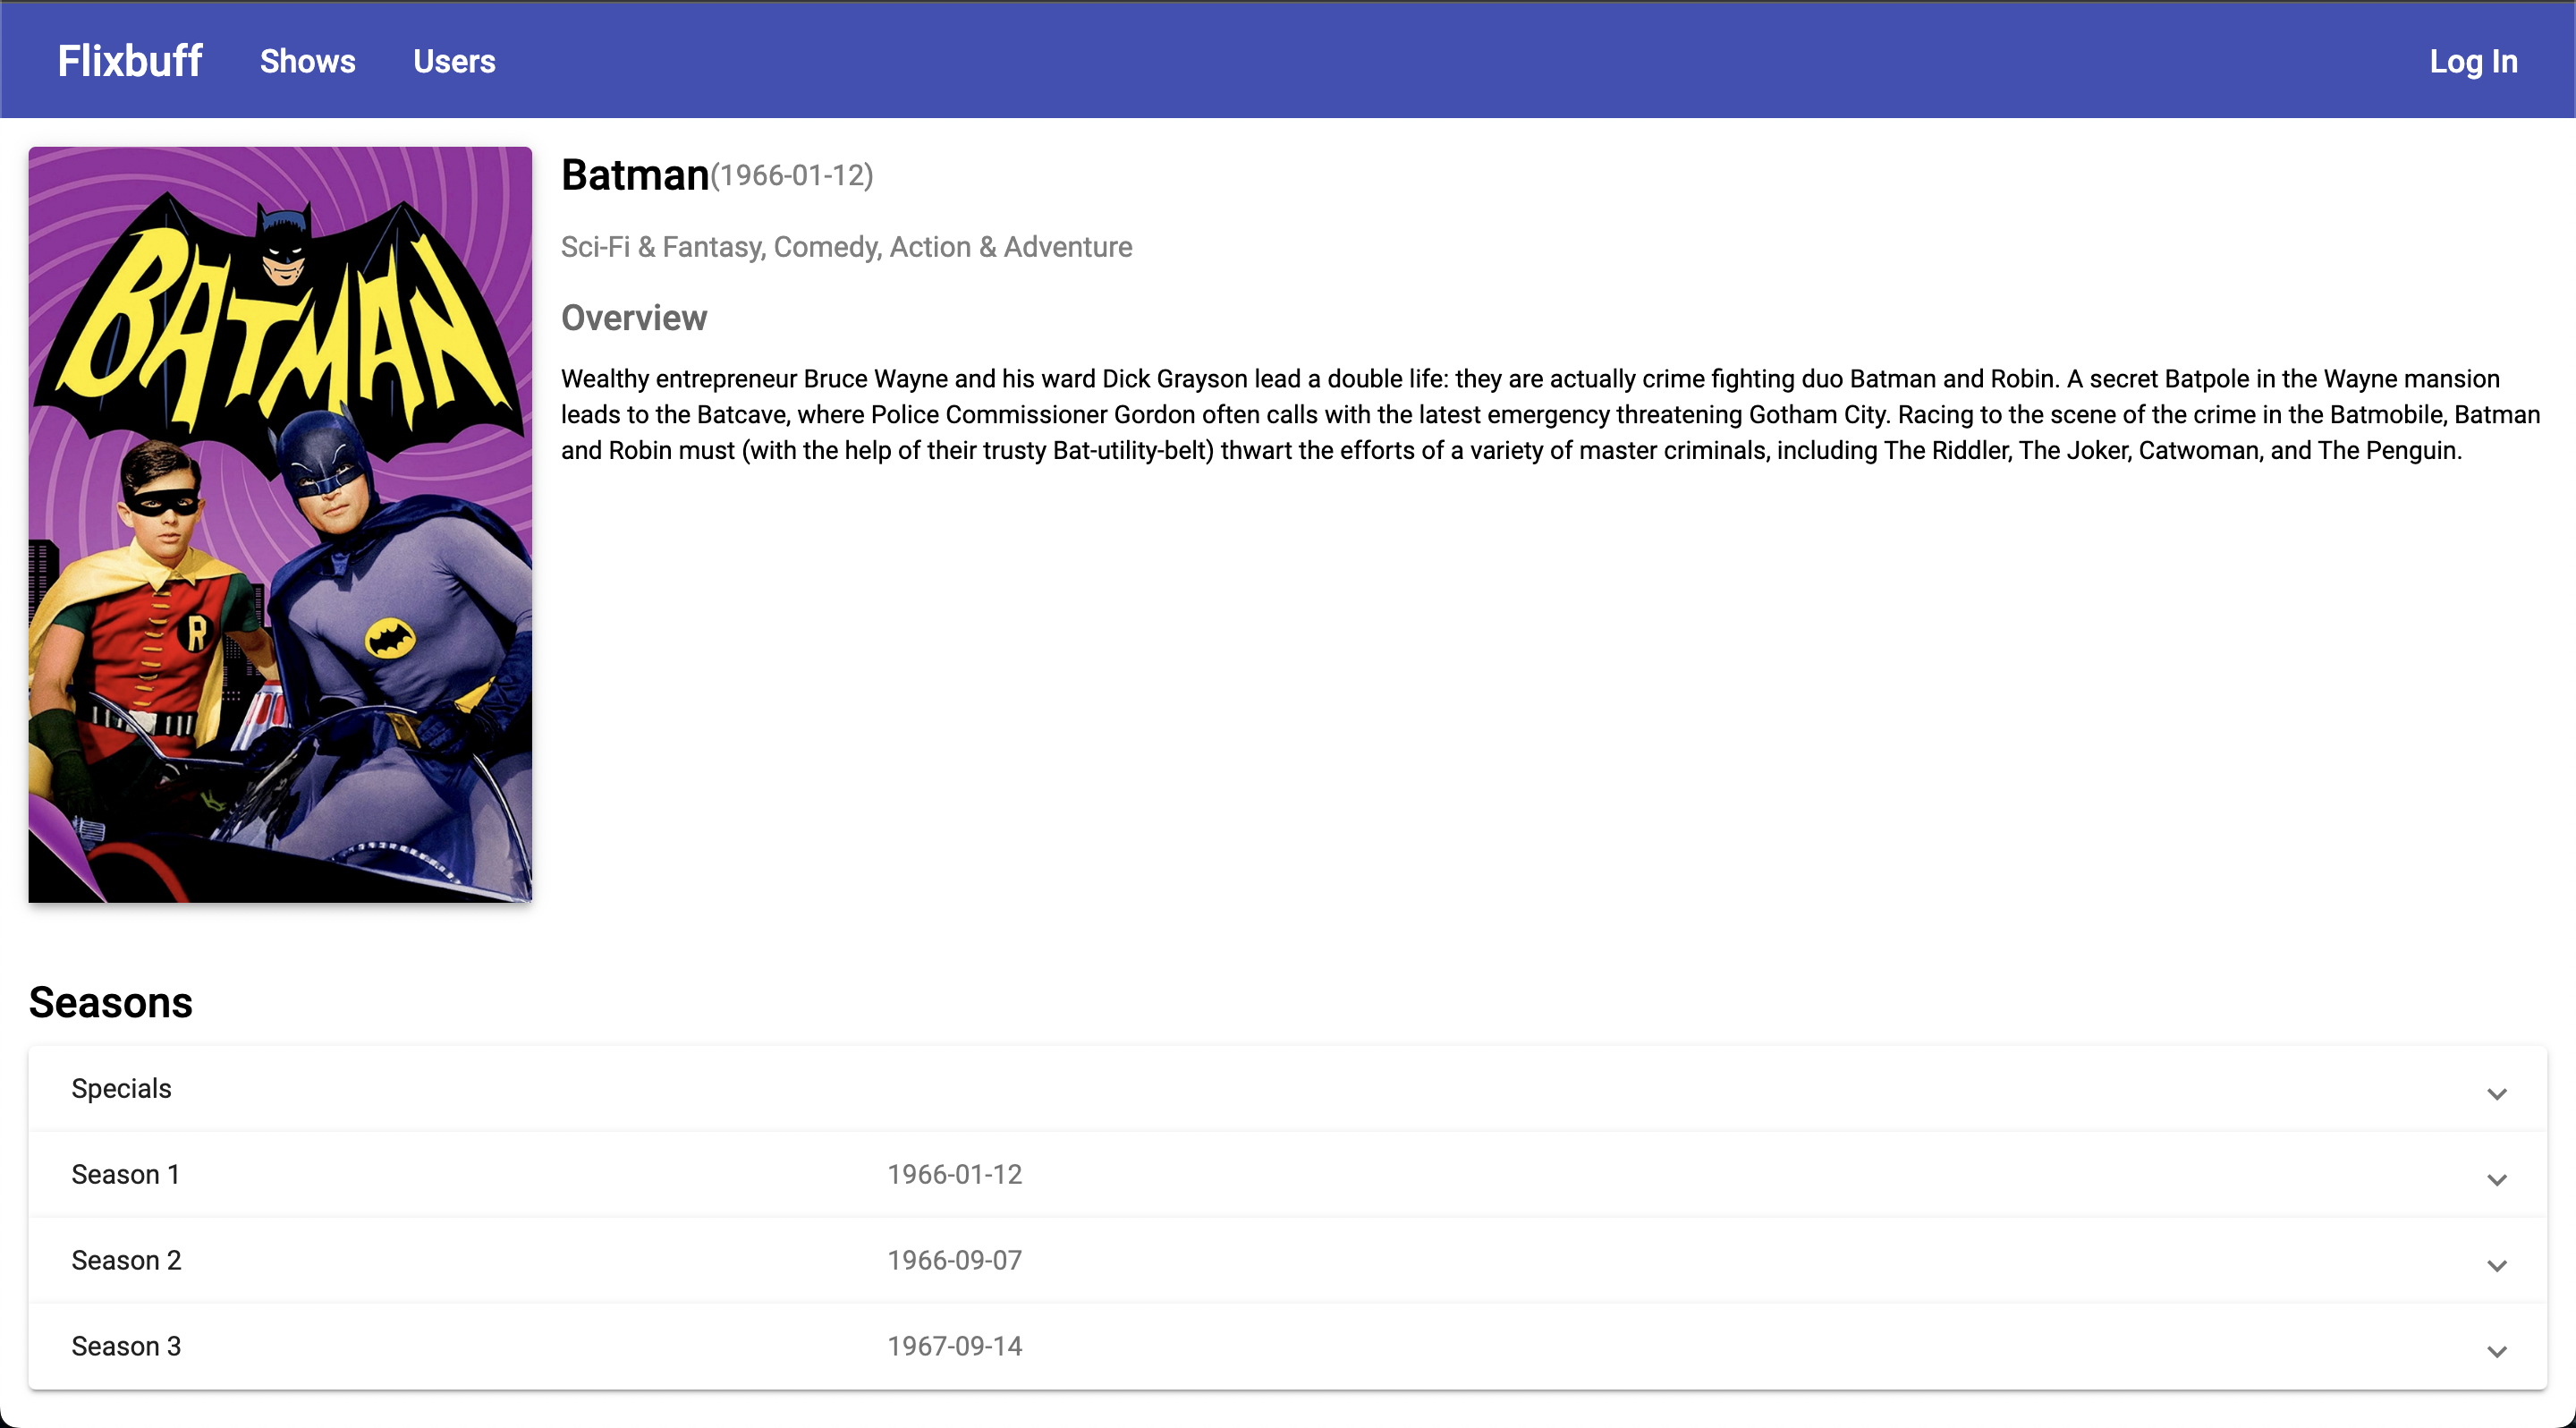
\includegraphics[scale=0.25]{img/show-details.png}
    \caption{ Detalles de la serie \textbf{Batman} }\label{fig:show-details}
\end{figure}

\begin{figure}[H]
    \centering	
        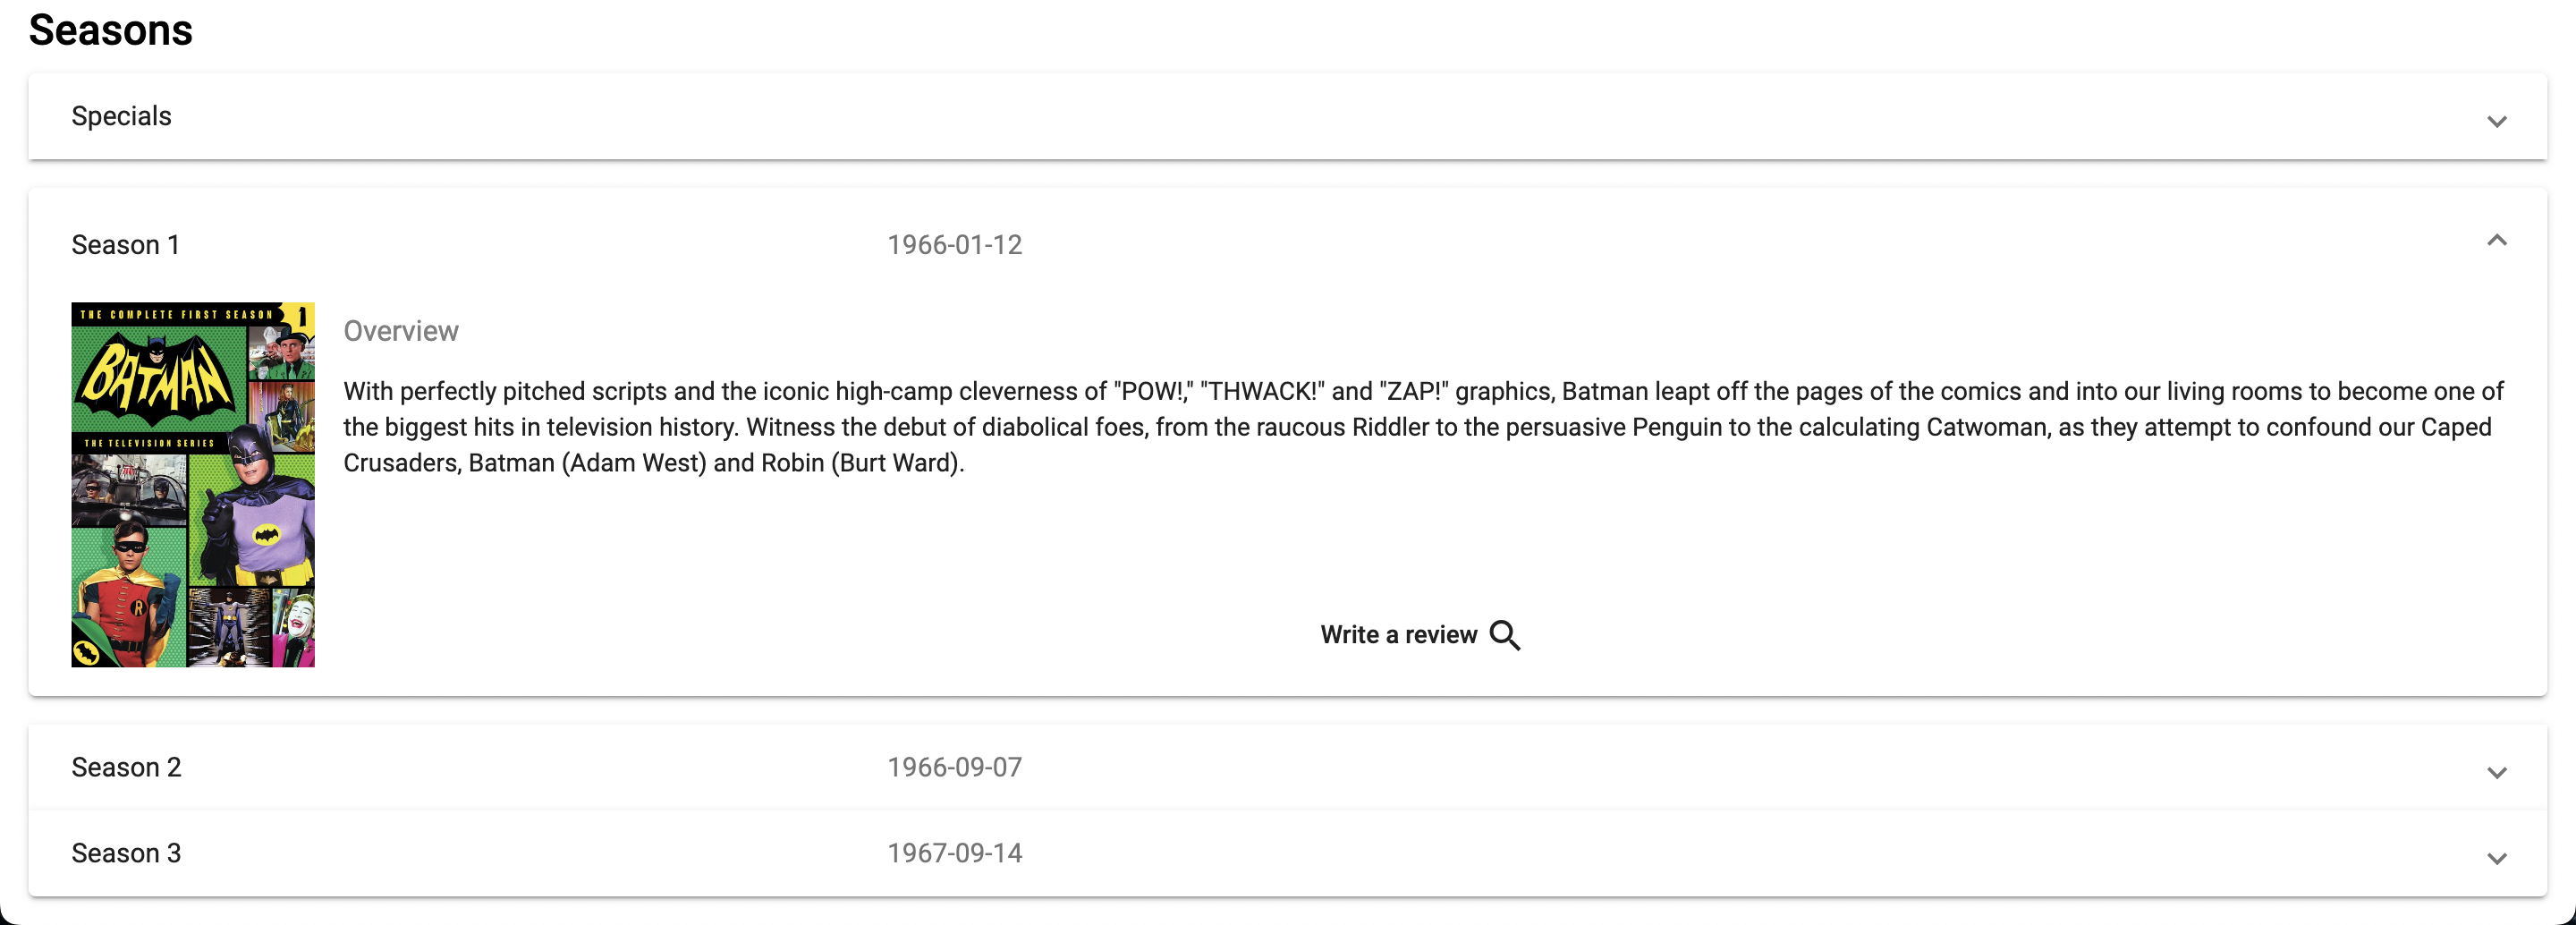
\includegraphics[scale=0.25]{img/expanded-season.png}
    \caption{ Lista de tarjetas de las temporadas de una serie }\label{fig:expanded-season}
\end{figure}

\subsubsection{Lista de usuarios}
Al igual que la lista de series, la lista de usuarios también se basa en una barra de búsqueda y unas tarjetas de
usuario. En este caso las tarjetas de usuario incluyen su nombre de perfil, el total de reseñas realizadas por el
usuario y el total de usuarios que le siguen. Haciendo click sobre ellas, navegas a la vista de detalles de ese
usuario.

\begin{figure}[H]
    \centering	
        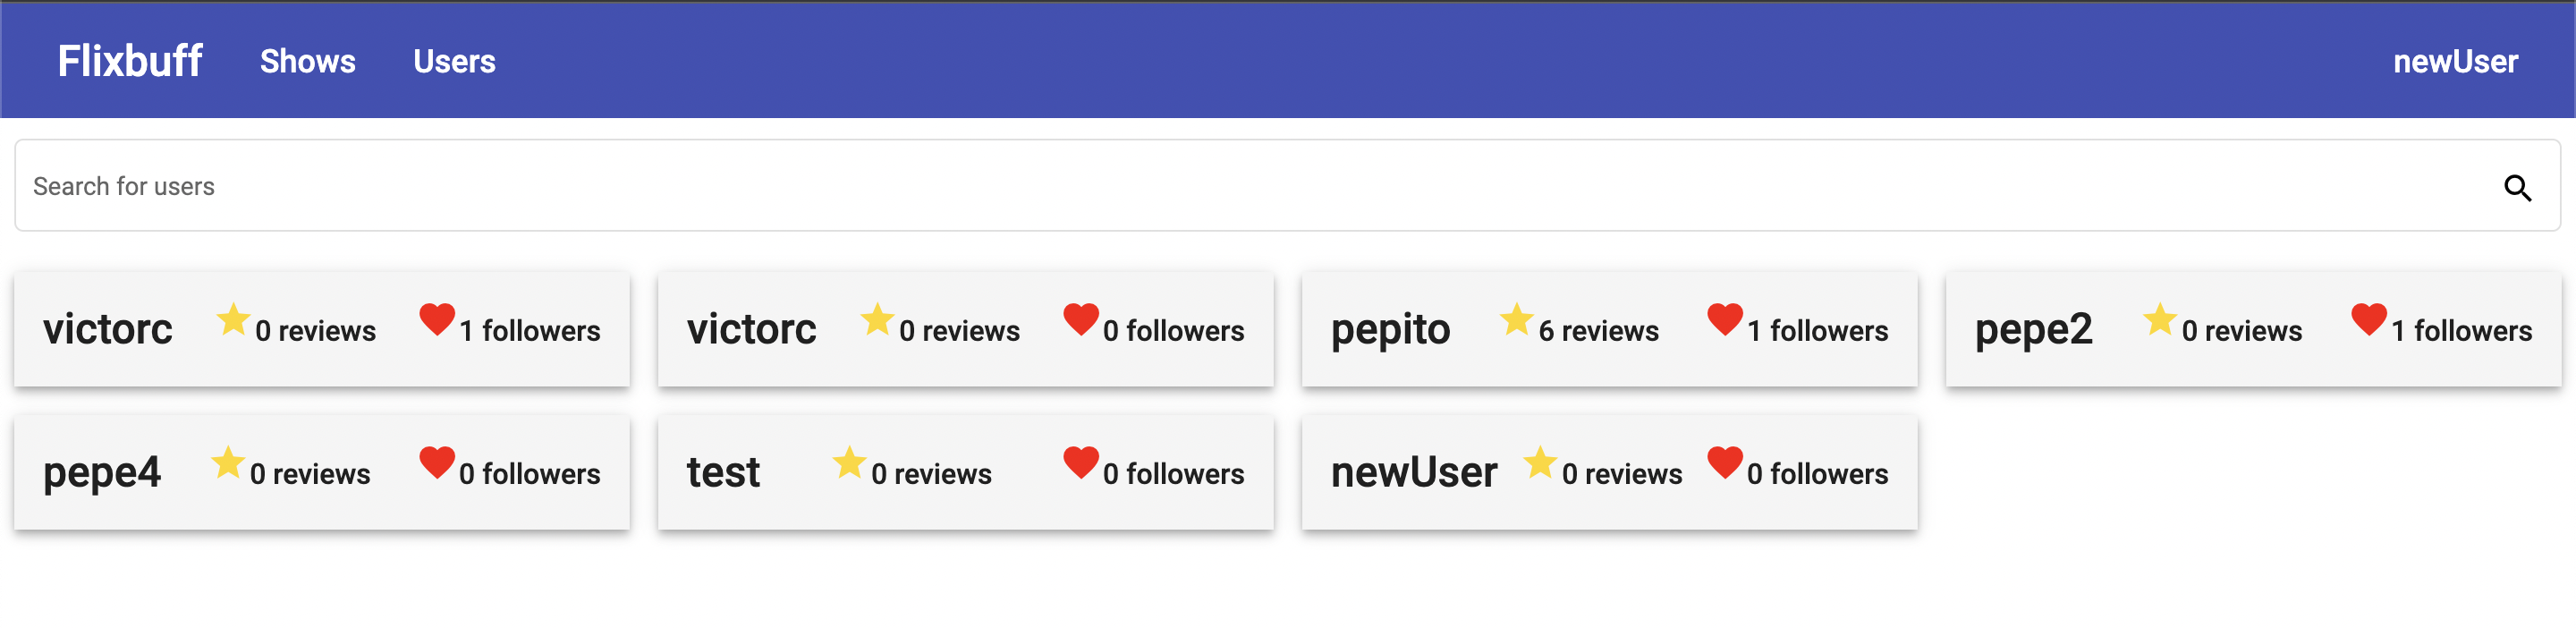
\includegraphics[scale=0.25]{img/user-list.png}
    \caption{ Lista de usuarios de la aplicación }\label{fig:user-list}
\end{figure}

\subsubsection{Detalles de un usuario}
La vista de detalles del usuario, muestra una rejilla de tarjetas, en las que se representan todas sus reseñas,
ordenadas de más a menos recientes.\\

En la esquina superior derecha, se muestra un botón de \textit{follow} a los usuarios logueados, para que puedan seguir
al usuario del que están viendo los detalles.

\begin{figure}[H]
    \centering	
        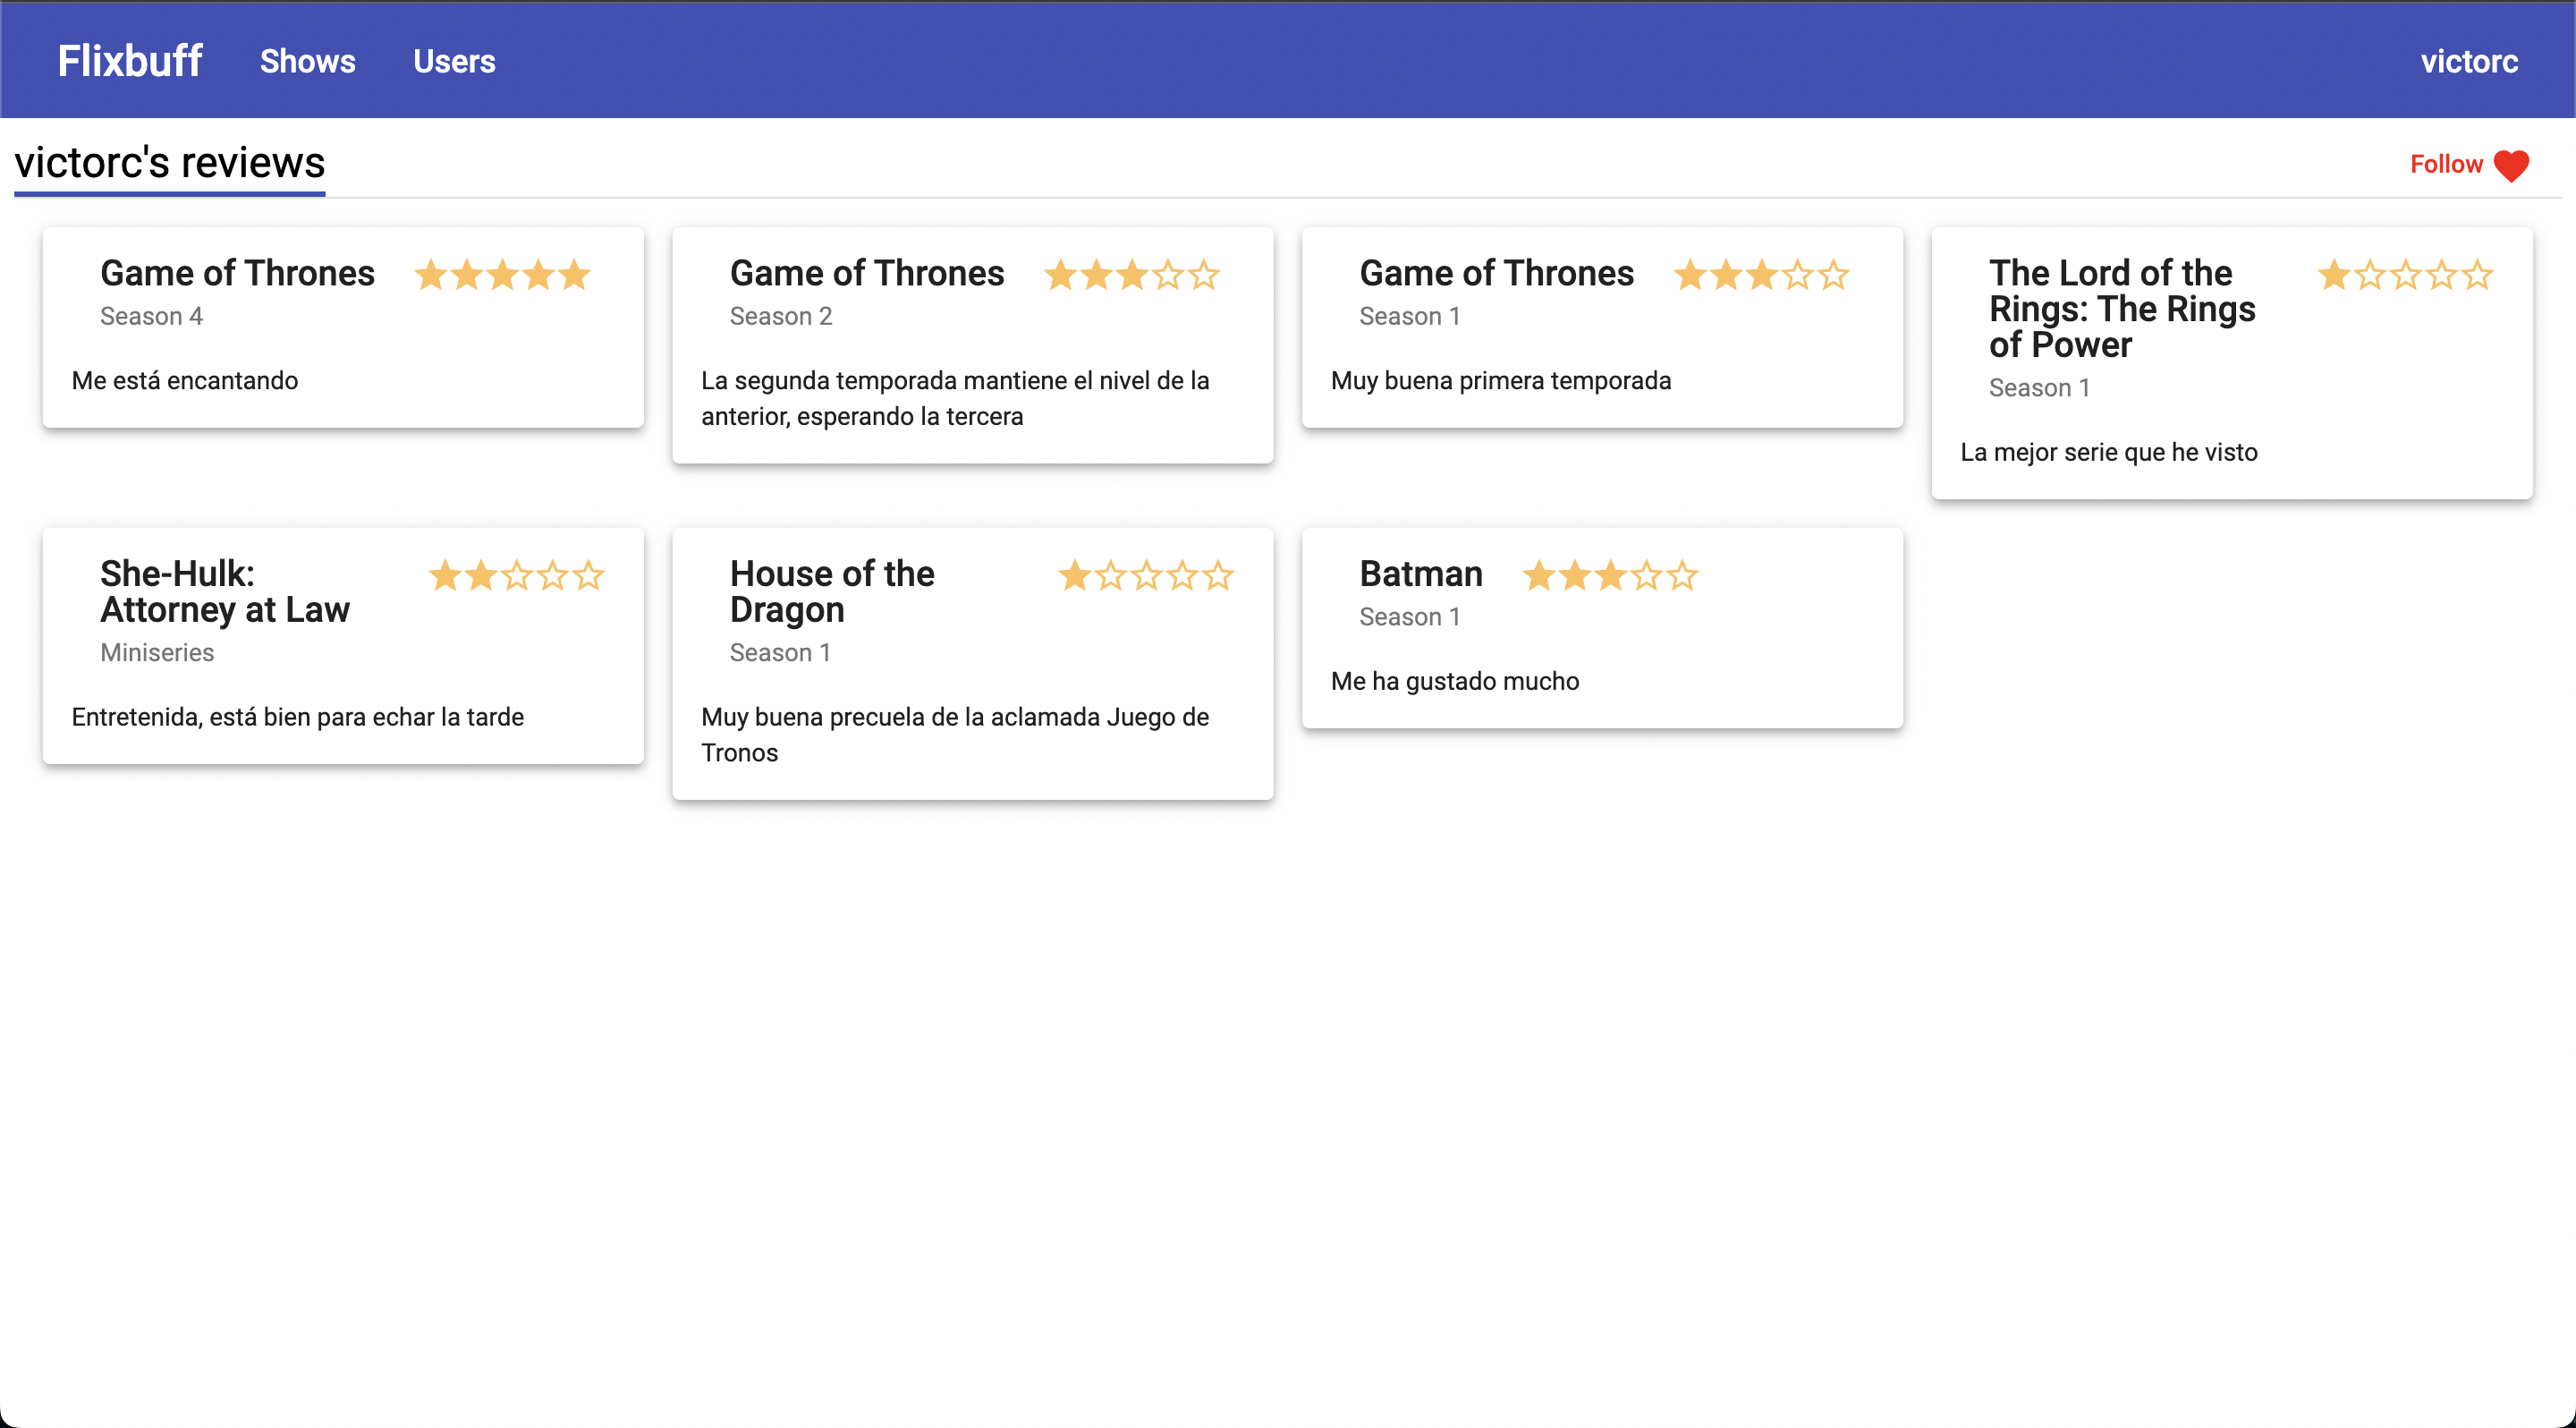
\includegraphics[scale=0.25]{img/user-details.png}
    \caption{ Detalles del usuario victorc }\label{fig:user-details}
\end{figure}

\section{Despliegue}\label{sec:despliegue}
Para el despliegue de la aplicación había infinidad de opciones en cuanto a servidores: montar un servidor en una
máquina de Ubuntu, \textit{AWS}\cite{aws}, \textit{Azure}\cite{azure}, etc.\\

Después de barajar las posibilidades hemos elegido \textit{Heroku}, una plataforma en la nube que nos permite montar un
servidor con nuestra aplicación, de forma muy sencilla e intuitiva, directamente desde nuestro repositorio en
\textit{GitHub}, permitiéndonos despliegues manuales o automáticos de cualquier rama del repositorio.\\

Para nuestra base de datos, hemos utilizado \textit{MongoAtlas}, de la que hablamos en secciones anteriores.

\subsection{Implementación del despliegue}
Hemos creado dos aplicaciones en la plataforma: una para servir la aplicación web y otra para la API.\\

Para desplegar el servidor, hemos necesitado instalar \textit{gunicorn}\cite{gunicorn}, que nos permite transformar
nuestra aplicación de \textit{flask} en un servidor HTTP. Además, hemos dado instrucciones a \textit{Heroku} a través de
un fichero \textit{Procfile} en el que se detalla cómo ejecutar el servidor con \textit{gunicorn}.

Por otra parte, para el despliegue del cliente, hemos creado un fichero \textit{server.js} que se ocupa de escuchar las
peticiones del puerto 8080 y devolverles los ficheros correspondientes. El resultado del despliegue se puede ver
\href{http://flixbuff-front.herokuapp.com/}{aquí}.\\

Al estar las aplicaciones dentro de subdirectorios en el repositorio, hemos utilizado un \textit{buildpack} para
\href{https://github.com/timanovsky/subdir-heroku-buildpack.git}{subdirectorios}, que nos permite establecer qué
subdirectorio de nuestro repositorio utilizar para el servidor, en lugar del repositorio completo.

\subsection{Costes del despliegue}\label{sec:costes-despliegue}
\subsubsection{Heroku}
\textit{Heroku} nos ofrece distintas \textit{tiers} de precios para alojar nuestra aplicación, desde una \textit{tier}
gratuita, hasta una \textit{tier} de altas prestaciones.\\

Dentro de cada \textit{tier} nos ofrece distintos \textit{dynos}, contenedores ligeros y aislados de Linux, en los que
se ejecuta tu aplicación. Cada uno de los distintos tipos de \textit{dyno}, tiene un precio distinto.

\begin{figure}[H]
    \centering	
        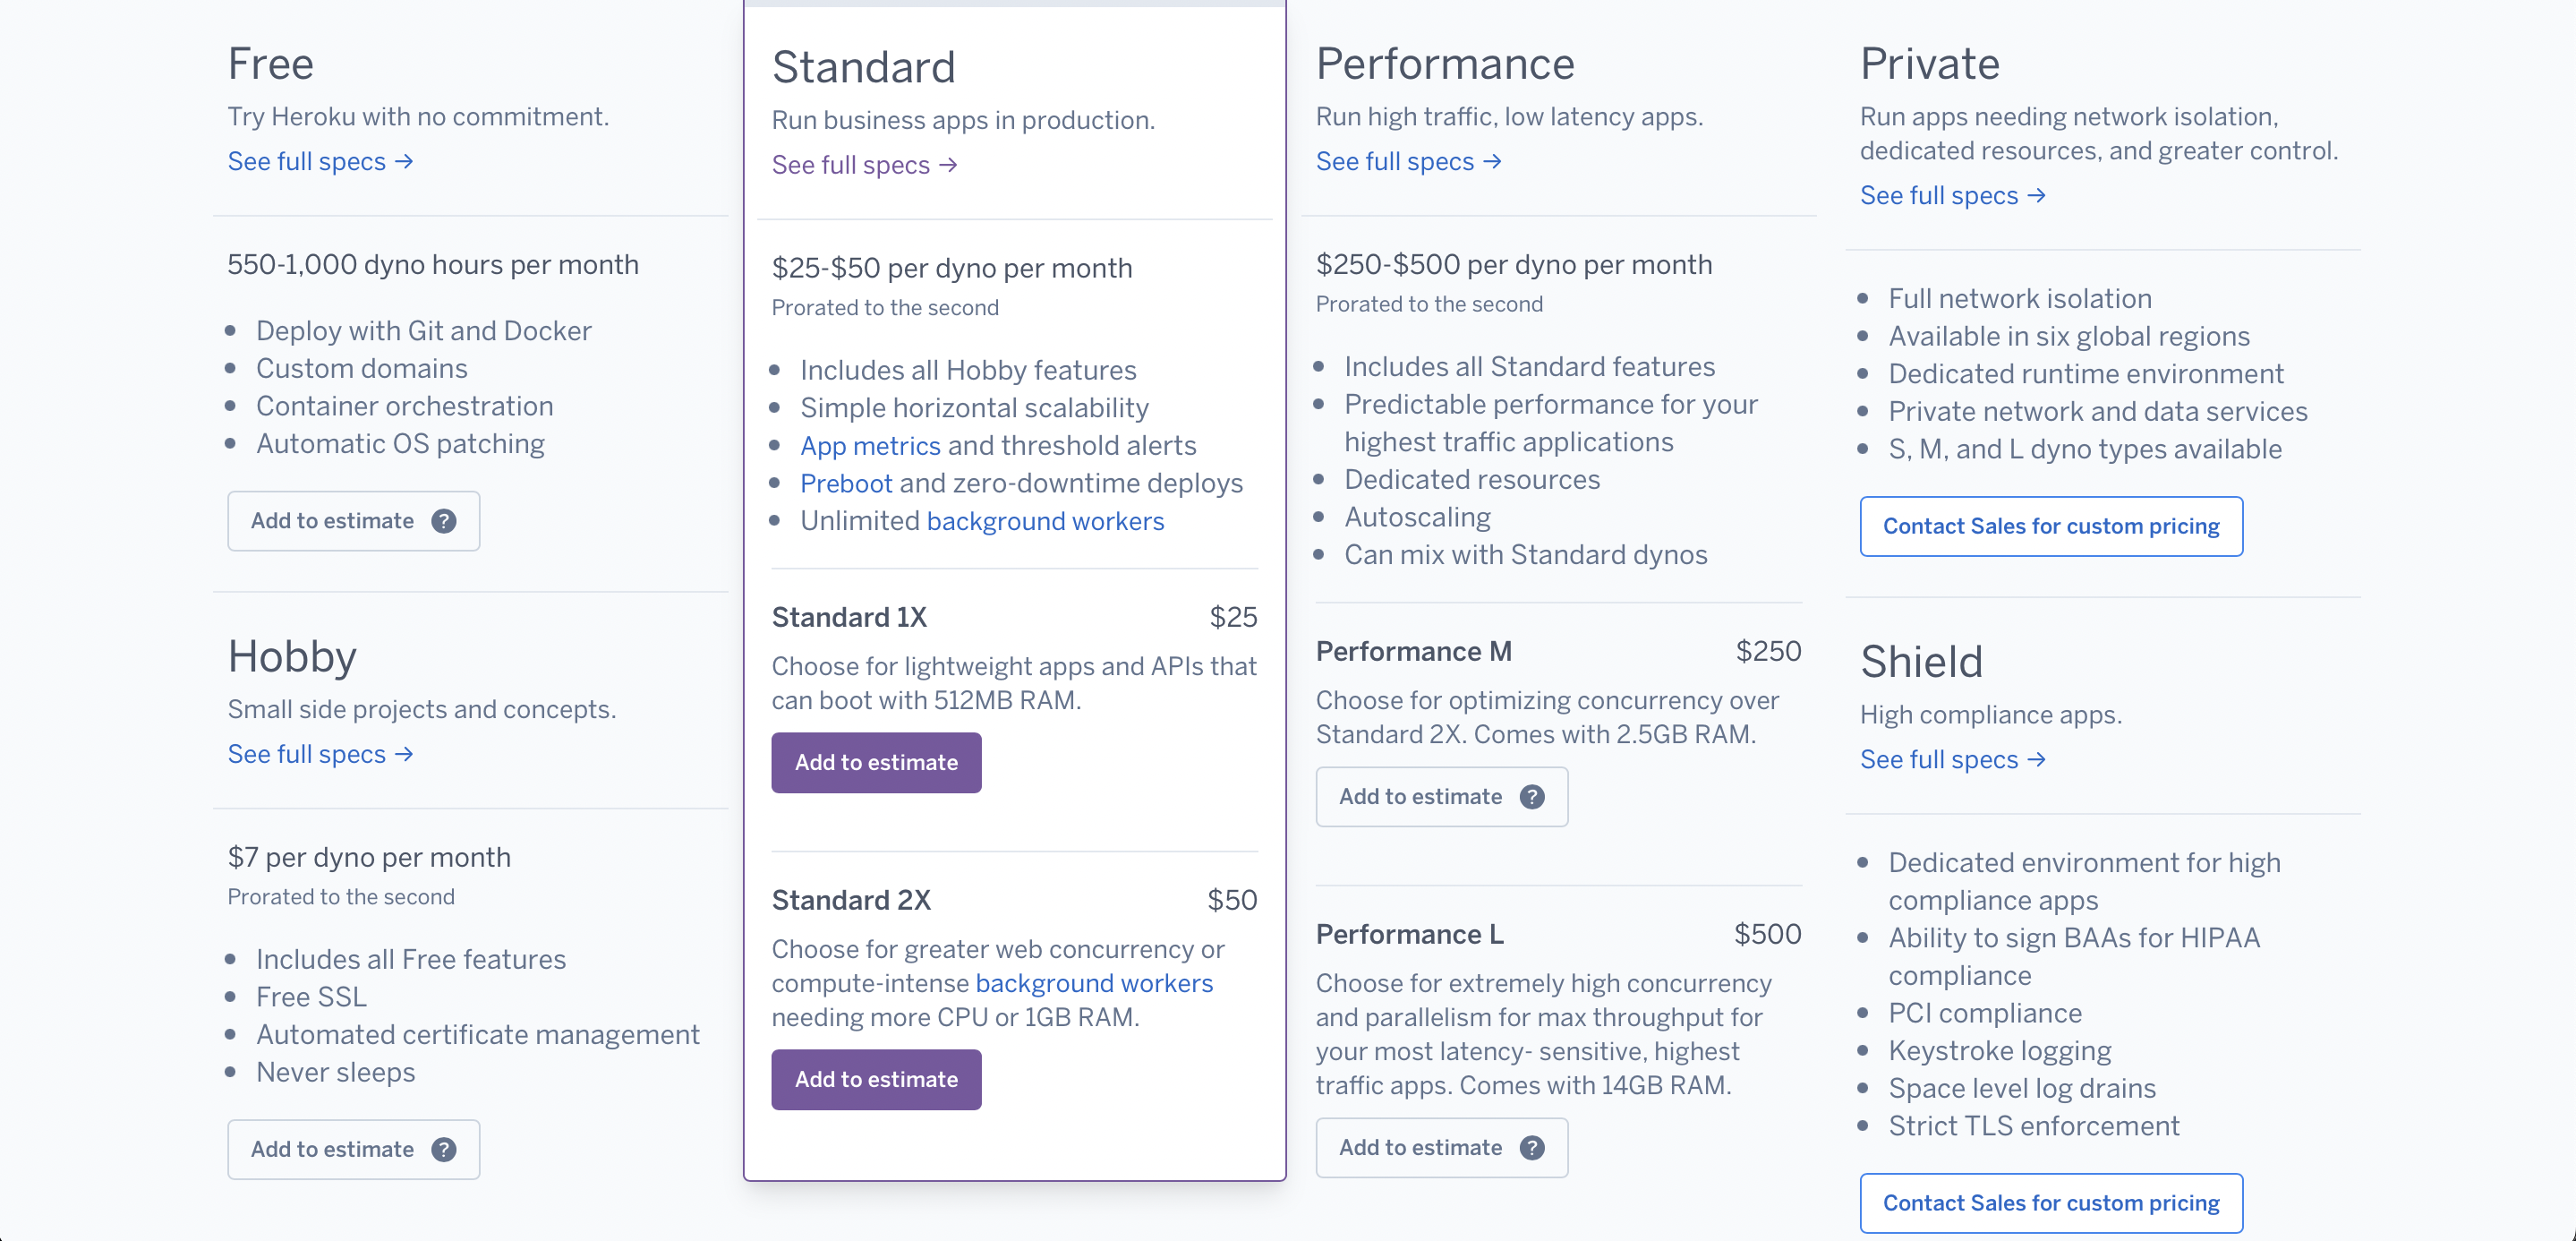
\includegraphics[scale=0.25]{img/heroku-tiers.png}
    \caption{ Precios de las \textit{tiers}/\textit{dynos} de \textit{Heroku} }\label{fig:heroku-tiers}
\end{figure}

En esta etapa del desarrollo del proyecto, elegiremos el \textit{tier} gratuito, ya que el proyecto aún está en
desarrollo.\\

Una de las ventajas de \textit{Heroku} es que nos permite fácilmente cambiar de \textit{tier} en el momento que
queramos, permitiéndonos escalar nuestra aplicación fácilmente.

\subsubsection{MongoAtlas}
Al igual que \textit{Heroku}, \textit{MongoAtlas} también nos ofrece diferentes planes y \textit{tiers}.\\

Cuenta con tres planes principales: \textit{serverless}, para aplicaciones con poco tráfico o simple almacenaje de
datos, \textit{dedicado}, el recomendado para aplicaciones en producción, y \textit{compartido}, para pruebas y 
aplicaciones en desarrollo.\\

Cada uno de los planes cuenta con diferentes \textit{tiers} de clústeres, cada uno con diferente precio y
prestaciones.\\

En nuestro caso, al igual que con el servidor de \textit{Heroku}, hemos optado por la opción gratuita, sabiendo que
podremos escalarla fácilmente desde la configuración de \textit{MongoAtlas}.

\begin{figure}[H]
    \centering	
        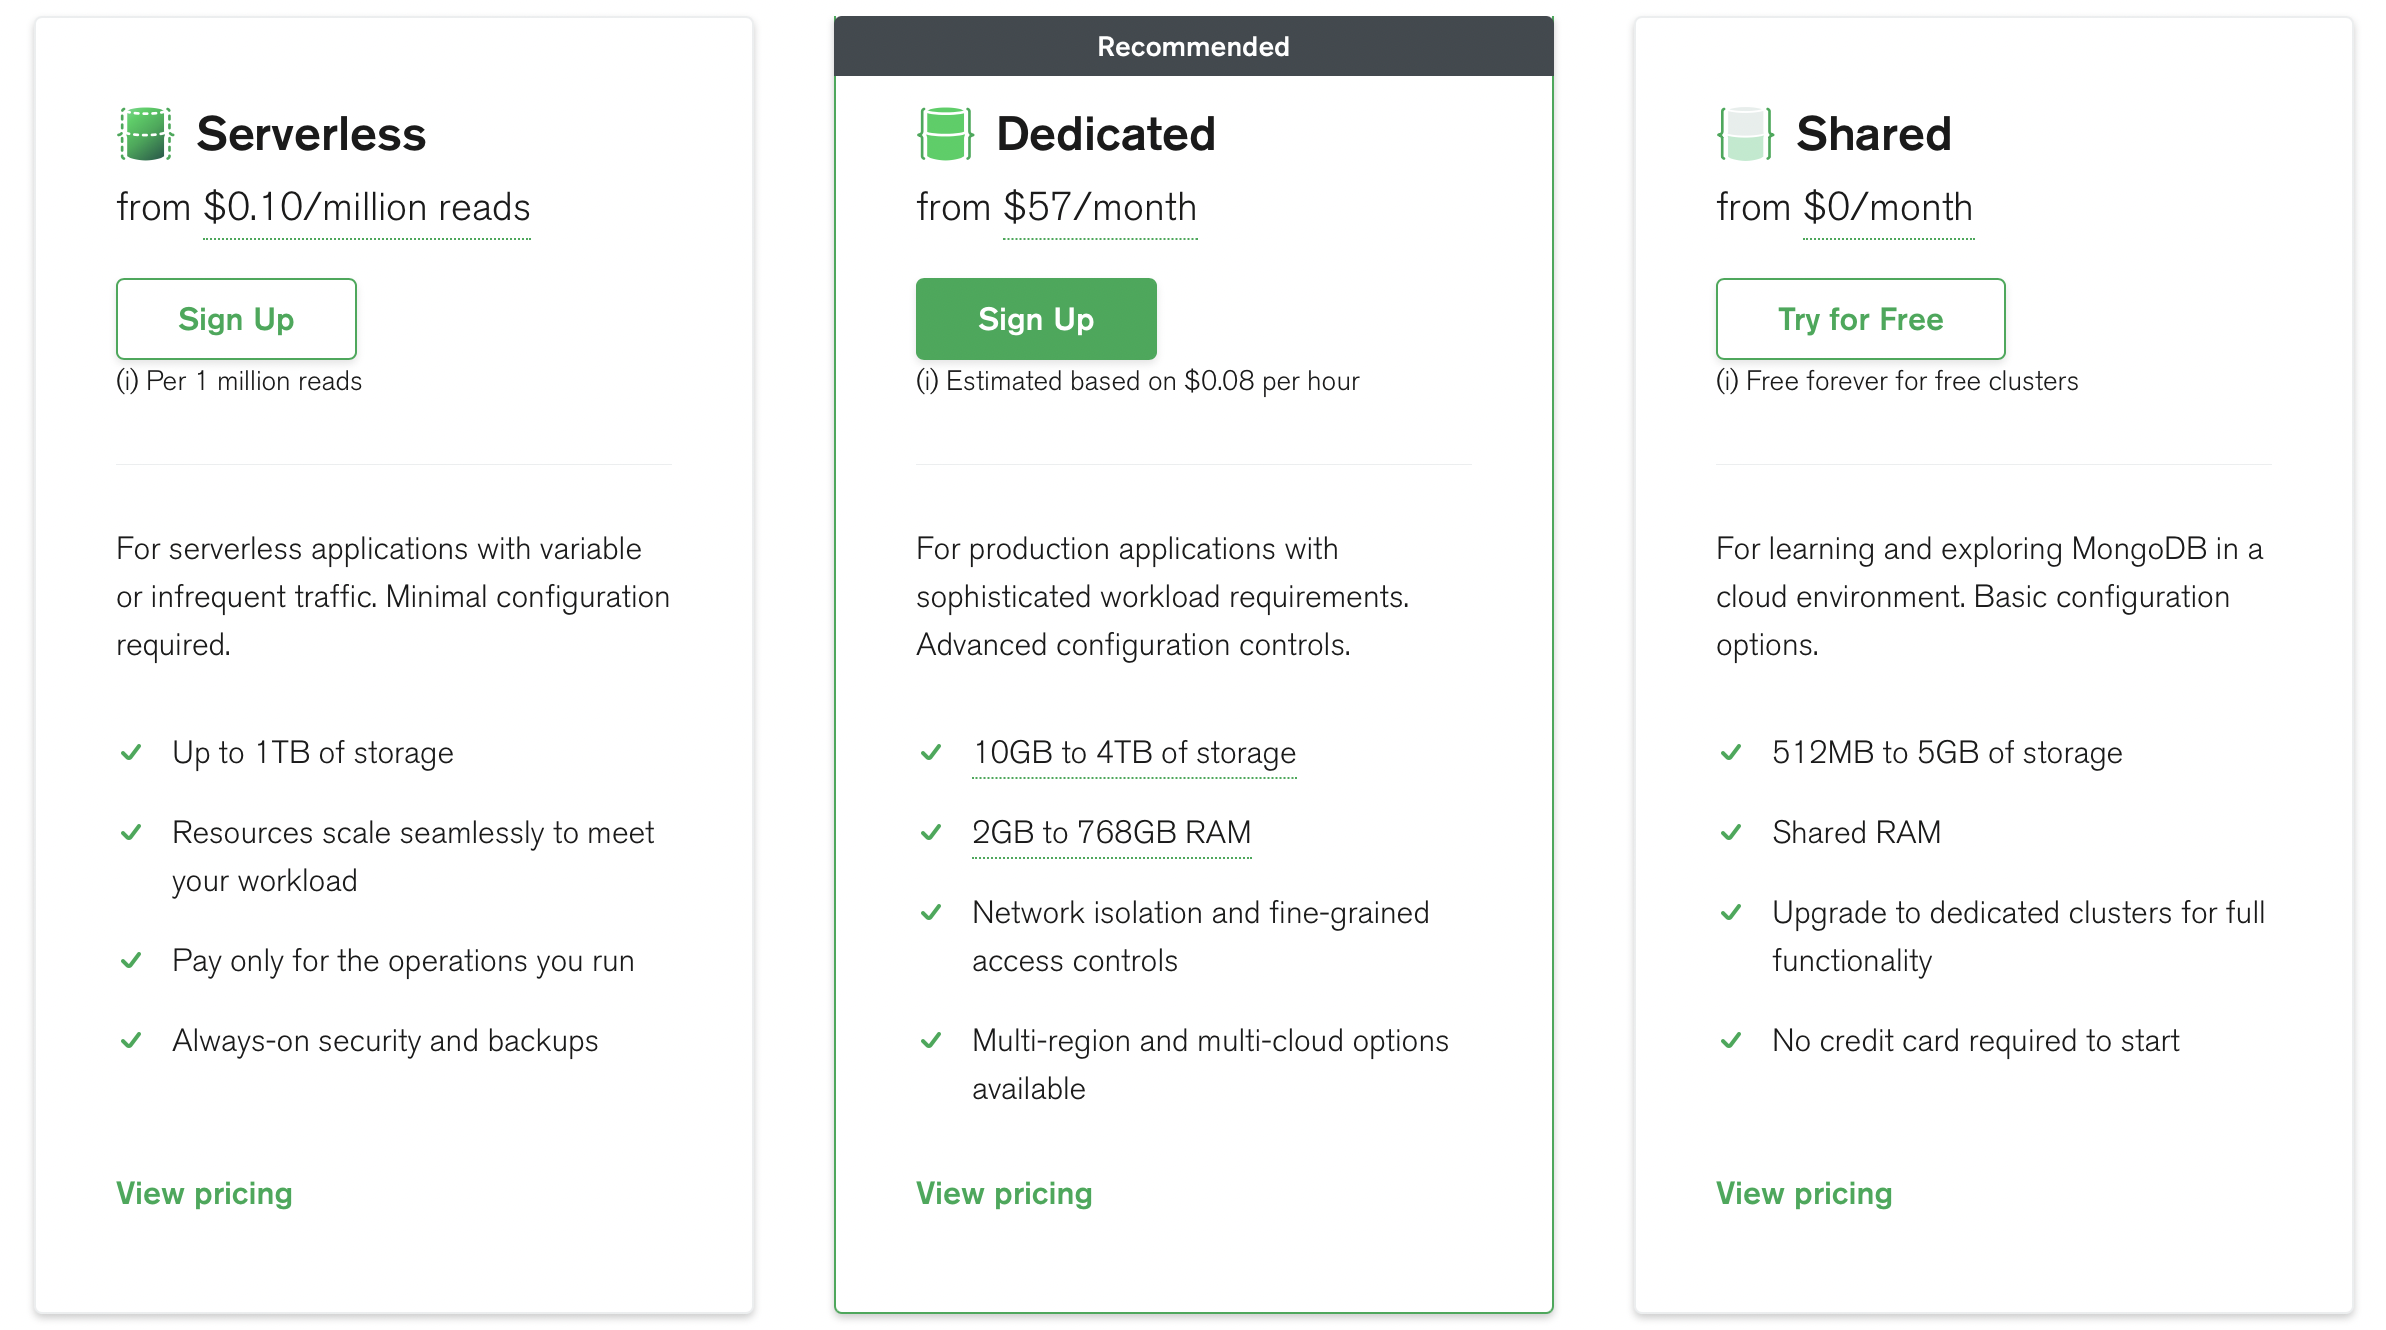
\includegraphics[scale=0.25]{img/mongo-plans.png}
    \caption{ Precios estimados de los distintos planes de \textit{MongoAtlas} }\label{fig:mongo-plans}
\end{figure}

\begin{figure}[H]
    \centering	
        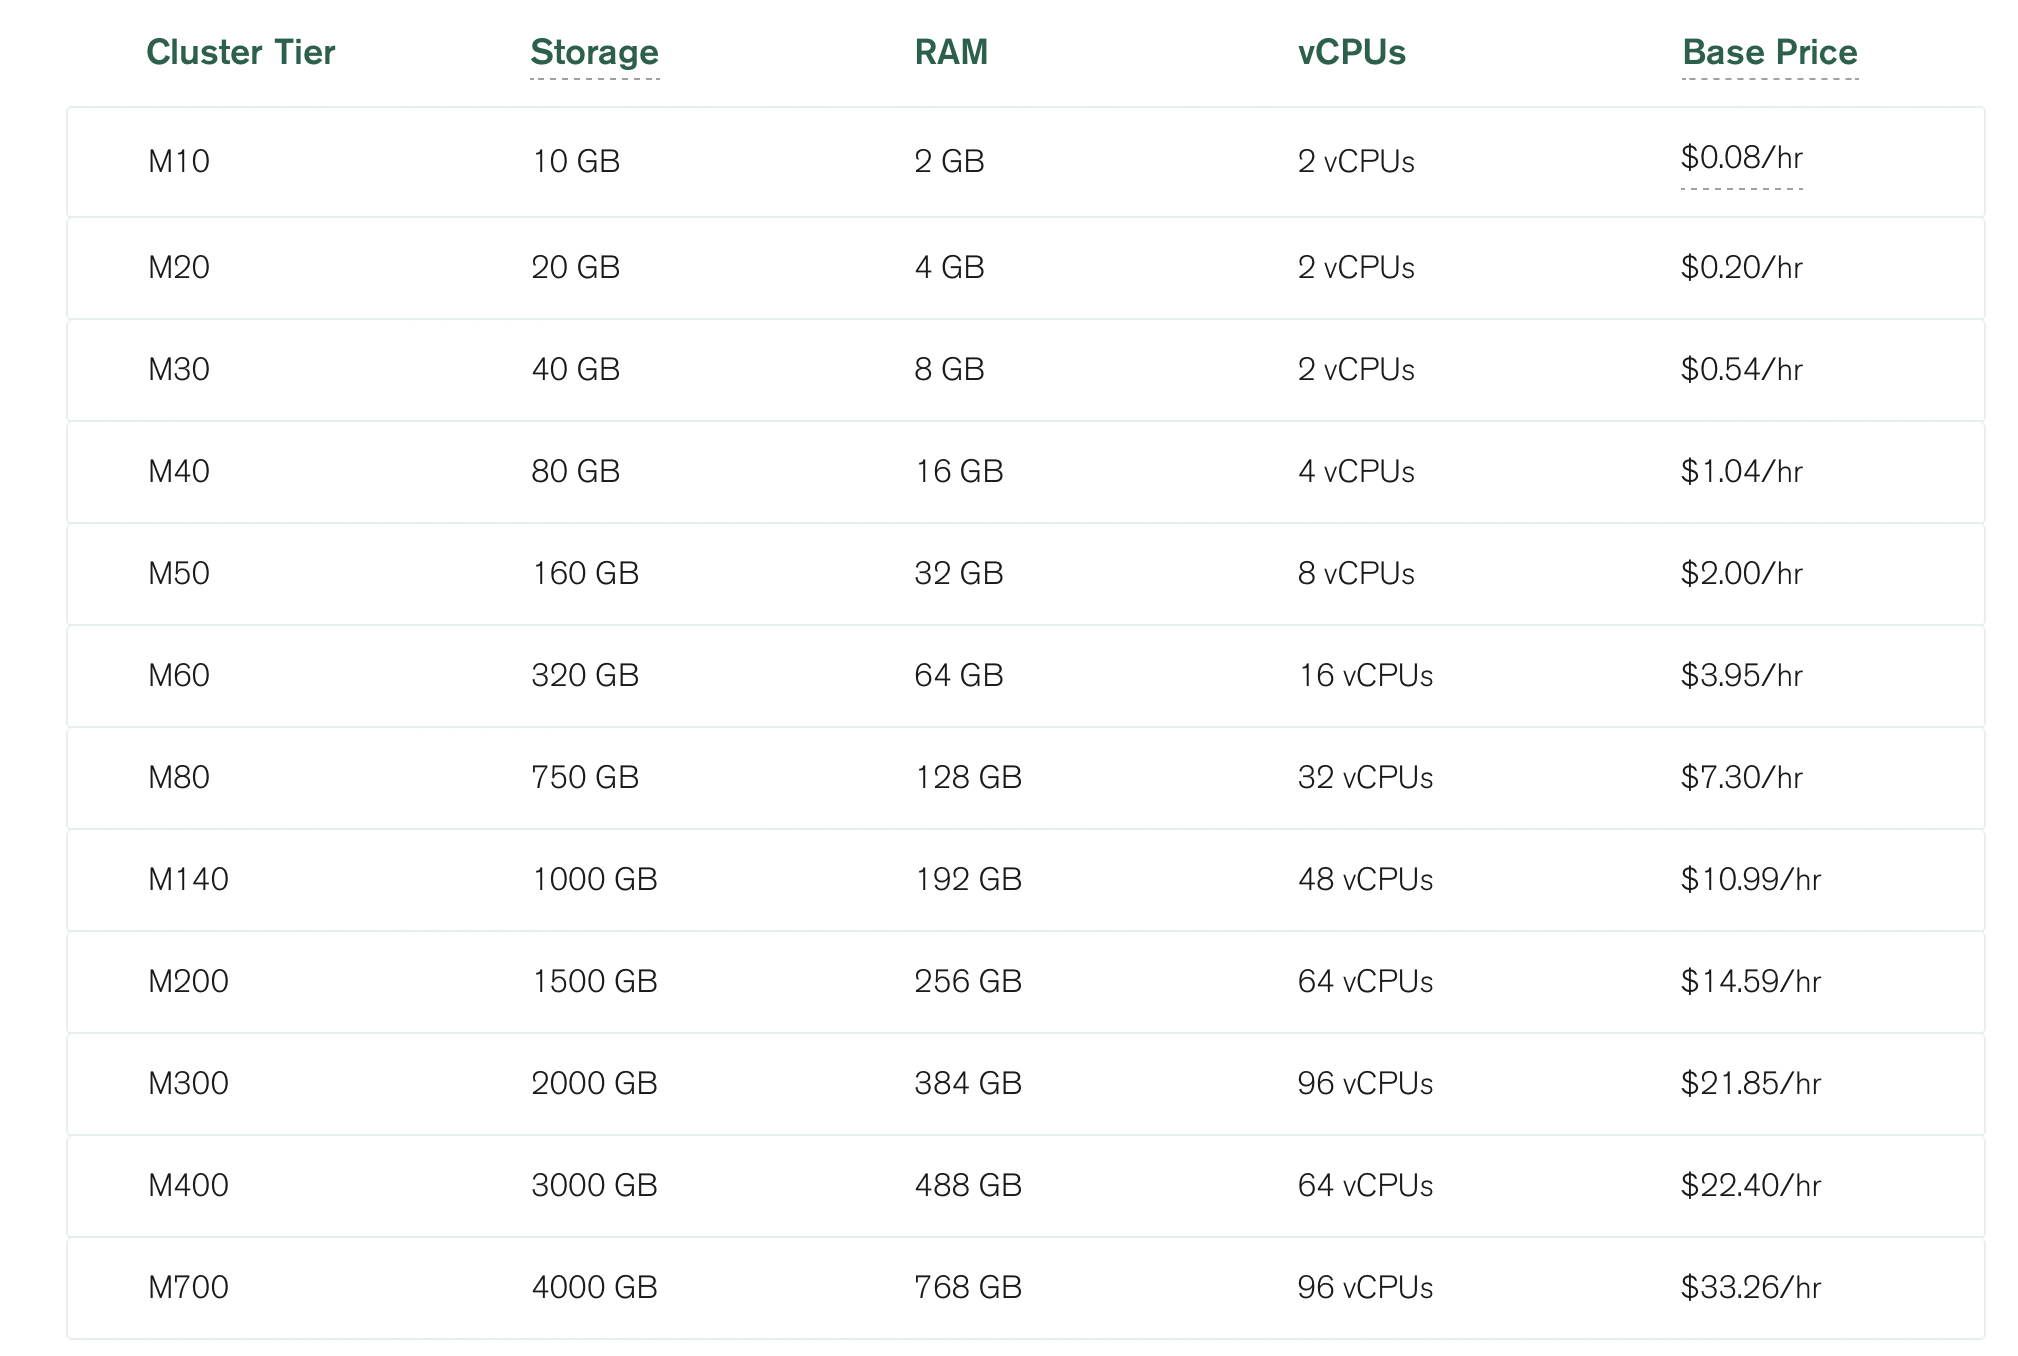
\includegraphics[scale=0.25]{img/mongo-tiers.png}
    \caption{ Precios de las \textit{tiers} de \textit{MongoAtlas} }\label{fig:mongo-tiers}
\end{figure}
